\documentclass[../ana1.tex]{subfiles}
\onlyinsubfile{\sectionNumbering} %Use numbering relative to sections and not subsection

\begin{document}
\setcounter{section}{14}
\section{Stetigkeit}
Sei \( D \subset \R^n, f \colon D \rightarrow \R^m, 
x \mapsto f(x) \) eine Funktion.\\
Im Fall \( m=1 \) heißt die Funktion reellwertig. 
Ist \( D = I \subset \R \) ein Intervall, so bezeichnet 
man \( C: I\rightarrow R^m \) als einen Weg oder auch Kurve.\\
z.\ B.\ 
\[ c(t) = (x(t), y(t), z(t)),\ t=\text{Zeit} \]

\begin{bspe}\leavevmode
    \begin{enumerate}
        \item horizontaler Wurf aus der Höhe \( h \) mit 
        Geschwindigkeit \(v\) \\
        Bild:
        \begin{center}
            \begin{tikzpicture}[scale=3]
                \draw[->] (0,-0.1) -- (0,1) node[above] {\(z\)};
                \draw[->] (-0.1,0) -- (1,0) node[right] {\(x\)};
                \draw (0.05,0.75) -- (-0.05,0.75) node[left] {\(h\)};
                \draw[thin,domain=0:0.866,smooth,variable=\t,black] plot ({\t},{0.75 - 1/2 * 2 * \t * \t});
            \end{tikzpicture}
        \end{center}
        \( c: \left[0, \sqrt{\frac{2 h}{g}} \, \right] \Rightarrow 
        \R^3, c(t) = (vt, 0, h - \frac{1}{2} g t^2) \)
        \item Abstand zu einer Menge \( E \subset \R^n \):\\
        \( \mathrm{dist}_E : \R^n \rightarrow \R, \mathrm{dist}_E(x) 
        := \inf \{ \abs{x-y} \;\vert \; y\in E \} \)
        \begin{center}
            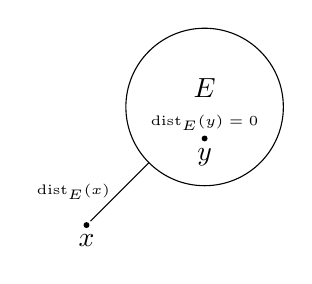
\begin{tikzpicture}
                \draw (0,0) node[above] {\(E\)} circle (1);
                \draw[fill=black] (-1.5,-1.5) node[below] {\(x\)} circle (0.03);
                \draw (-1.5 + 0.05,-1.5 + 0.05) -- (-0.707, -0.707)
                node[midway, left] {\tiny\( \mathrm{dist}_E(x) \)};
                \draw[fill=black] (0,-0.4) node[below] {\(y\)} circle (0.03);
                \draw (0,-0.2) node {\tiny\( \mathrm{dist}_E(y) = 0 \)};
            \end{tikzpicture}
        \end{center}
    \end{enumerate}
\end{bspe}
\begin{defi}[Stetigkeit]
    Die Funktion \( f: D\rightarrow \R^m \) ist stetig 
    in \( x_0 \in D \), falls
    \[ \forall \, \varepsilon > 0 \,\exists \, \delta > 0 
    \, \colon \, \underbrace{ \abs{ f(x) - f(x_0) 
    }}_{\text{Abstand in } \R^m} < \varepsilon \quad 
    \forall x\in D \text{ mit } \underbrace{\abs{x - x_0} 
    }_{\text{Abstand in } \R^n} < \delta. \]
    \( f: D\rightarrow \R^m \) heißt stetig, falls \( f \) 
    stetig in allen \(x_0 \in D \) ist.
\end{defi}
\begin{bem}
    Mittels der Bälle 
    \[ B_r^d(y_0) := \{ y\in\R^d \;\colon \; 
    \abs{y-y_0}<r \} \]
    kann man Stetigkeit von \( f \) in \( x_0 \) auch wie folgt
    auffassen.
    \[ \forall \, \varepsilon > 0 \,\exists \, \delta > 0 
    \;\colon \; f(D\cap B_\delta^n(x_0)) \subset 
    B_\varepsilon^m (f(x_0)) \]
\end{bem}
\begin{bspe}\leavevmode
    \begin{enumerate}
        \item Die konstante Funktion \( f: D\rightarrow \R^m, 
        x\mapsto c\in\R^m \) fest.
        Sei \( x_1\in D \)
        \[ \Rightarrow f(x) - f(x_2) = c - c = 0 \]
        \[ \Rightarrow \abs{f(x_1) - f(x_2)} = 0 \quad \forall \, 
        x_2\in D \]
        \(\Rightarrow f\) ist stetig.
        \item \( a\in\R, f:\R \rightarrow \R, x\mapsto ax \)
        \[ \Rightarrow \abs{ f(x) - f(x_0) } = 
        \abs{ ax - ax_0 } = \abs{a}\abs{x-x_0} \]
        \[ \Rightarrow \text{Wähle }\delta = 
        \frac{\varepsilon}{1+\abs{a}} 
        \ (a=0 \text{ ist erlaubt}) \]
        \[ \Rightarrow \abs{f(x) - f(x_0)} = \abs{a}
        \abs{x-x_0} < \abs{a} \frac{\varepsilon}{1+\abs{a}}
        < \varepsilon \quad \forall \abs{x-x_0} < \delta. \]
        Somit ist \(f\) stetig in \(x_0\).
        \item \( f:\R\rightarrow\R, x\mapsto x^2 \)
        ist stetig, denn
        \begin{align*}
            \abs{ f(x) - f(x_0) } &= \abs{x^2 - x_0^2} 
        = \abs{ (x+x_0)(x-x_0) }\\
            &\leq \underbrace{( \abs{x} + \abs{x_0} )}_{
                \leq 2\abs{x_0}+1, \text{ falls } \abs{x-x_0} < 1
            } \abs{x-x_0}
        \end{align*}
        Zu \( \varepsilon > 0 \) und \( x_0 \in\R \) wähle
        \[ \delta := \min \left(1, \frac{\varepsilon}{1 + 2\abs{x_0}} \right)
        = \delta(\varepsilon, x_0) > 0 \]
        \begin{align*}
            \Rightarrow &\abs{ f(x) - f(x_0) }\\
            = &\abs{x^2 - x_0^2}\\
            \leq &(2\abs{x_0} + 1) \abs{x-x_0}\\
            < &\varepsilon \quad \forall \, \abs{x-x_0} < \delta.
        \end{align*}
        Also ist \(f\) stetig in jedem \( x_0\in\R \).
        \item Indikatorfunktion 
        \[ E\subset \R, 
        \mathds{1}_E : \R\rightarrow\R, x\mapsto 
        \begin{cases}
            1, x\in E\\
            0, x\in\R \setminus E
        \end{cases} \]
        Sei \( \mathds{1} \) stetig in \( x_0\in E \). Dann existiert
        \( \varepsilon = \frac{1}{2} \) ein \(\delta > 0\) so, dass
        \[ \abs{ \mathds{1}_E(x) - \mathds{1}_E(x_0) } < \frac{1}{2} 
        \quad \forall x\in (x_0 - \delta, x_0 + \delta) . \]
        Ist \( \mathds{1}_E(x_0) = 1 \Rightarrow \mathds{1}_E(x) = 1 \)
        somit \( (x_0 - \delta, x_0 + \delta) \subset E \).\\
        Ist \( \mathds{1}_E(x_0) = 0 \Rightarrow \mathds{1}_E(x) = 0 \)
        somit \( (x_0 - \delta, x_0 + \delta) \subset E \).\\
        Spezialfall \( E = \Q, \mathds{1}_\Q \) heißt Dirichletfunktion.\\
        Fakt: \( \Q \) ist dicht in \( \R \), d.\ h.\ in jedem Intervall
        \( (x_0 - \delta, x_0 + \delta) \) für \( x_0 \in\Q \) gibt es
        reelle Zahlen.\\
        Andererseits ist die Menge \( \R\setminus\Q \) auch dicht in \(\R \), 
        denn \( \sqrt{2} \notin \Q \) und \( \sqrt{2}+\Q \subset \R\setminus\Q \) \\
        \( \Rightarrow \) im Intervall \( (x_0 - \delta, x_0 + \delta) \)
        gibt es Punkte aus \( \R\setminus\Q \) \\
        \( \Rightarrow \) die Dirichletfunktion \( \mathds{1}_\Q \) ist
        in jedem Punkt \( x_0 \in\R \) unstetig. 
        \item \[ x\in \R^d, \abs{x} = 
        {\left( \sum_{j=1}^d \abs{x_j}^2 \right)}^{\nicefrac{1}{2}} \]
        \( f:\R^d \rightarrow \R, x\mapsto \abs{x} \) ist stetig, denn
        \[ \abs{ f(x) - f(x_0) } = \abs{ \abs{x} - \abs{x_0} } 
        \overunderset{\text{Umgekehrte}}{\text{Dreiecksungl.}}{\leq} \abs{x - x_0}. \]
    \end{enumerate}
\end{bspe}
\begin{satz}[Folgenkriterium für Stetigkeit]
    Sei \( D\subset \R^n, f:D\rightarrow \R^m, x_0 \in D \). Dann sind
    äquivalent
    \begin{enumerate}
        \item \( f \) ist stetig in \( x_0 \).
        \item Für jede Folge \( {(x_k)}_{k\in\N} \) mit \( x_k \in D \)
        und \( \limes{k} x_k = x_0 \) folgt 
        \[ \limes{k} f(x_k) = f(x_0) \]
        (d.\ h.\  \( f(\limes{k} x_k) = \limes{k} f(x_k) \))
    \end{enumerate}
\end{satz}
\begin{bew}\leavevmode \\
    1. \(\Rightarrow \) 2. Sei \(x_k \in D \) und \( x_k 
    \rightarrow x_0 \) für \( k\rightarrow \infty \).
    Zu \( \varepsilon > 0 \) wähle man \( \delta > 0 \) mit
    \[ \abs{ f(x) - f(x_0) } < \varepsilon \quad \forall \, x\in D 
    \text{ mit } \abs{x-x_0}<\delta. \]
    \[ \Rightarrow \abs{ f(x_k) - f(x_0) } < \varepsilon
    \text{ für fast alle } k\in\N \]
    \[ \Rightarrow \limes{k} \abs{ f(x_k) - f(x_0) } = 0. \]
    2. \(\Rightarrow \) 1. Kontraposition. Sei \( f \) nichtstetig
    in \( x_0 \in D \).\\
    Dann gibt es ein \( \varepsilon > 0 \)
    \[ \forall \, \delta > 0 \,\exists \, x\in D : \abs{x-x_0} 
    < \delta : \abs{ f(x) - f(x_0) } \geq \varepsilon.\ (*) \]
    Wähle \( \delta = \frac{1}{n} \overset{(*)}{\Rightarrow}
    \exists \) Folge \( {(x_n)}_n, x_n \in D, x_n \rightarrow x_0 \)
    mit \( \abs{ f(x_n) - f(x_0) } \geq \varepsilon. \)
    \[ \Rightarrow f(x_n) \text{ konvergiert nicht gegen } f(x_0). \]
    \[ \neg 1. \Rightarrow \neg 2.\text{, d.\ h.\ }2.\Rightarrow 1. \]
\end{bew}
\begin{satz}[Verkettung]
    Seien \( f:D\rightarrow \R^m, f(D) \subset E \in\R^m, 
    g: E\rightarrow\R^k \). Ist \( f \) stetig in \( x_0 \)
    und \( g \) stetig in \( y_0 := f(x_0) \), so ist 
    \( g \circ f : D\rightarrow \R^k, x \mapsto (g\circ f)(x) 
    = g(f(x)) \) stetig in \( x_0 \).
\end{satz}
\begin{bew}
    Sei \( {(x_n)}_n \) eine Folge in \( D \) mit 
    \( x_n \rightarrow x_0 \).
    \[ \overset{\text{Satz 2}}{\Rightarrow} f(x_n) \rightarrow f(x_0)
    = y_0 \text{, da } f \text{ stetig ist.} \]
    \[ \overset{\text{Satz 2}}{\Rightarrow} g(f(x_n))
    \rightarrow g(y_0) = g(f(x_0)) \text{, da } g \text{ stetig ist.} \]
    \[ \overset{\text{Satz 2}}{\Rightarrow} g\circ f 
    \text{ ist stetig in } x_0. \]
\end{bew}
\begin{bsp}
    Sei \( f,g : D\rightarrow \R \) stetig. Dann sind auch
    \[ \abs{f} : D \rightarrow \R, x\mapsto \abs{f(x)} \]
    und
    \[ \max(f,g) = \frac{1}{2} (f+g + \abs{f-g}) \text{ und } \min(f,g) = \frac{1}{2} (f+g - \abs{f-g} ) \]
    stetig.
\end{bsp}
\begin{lem}
    Eine Funktion \[ f: D\rightarrow \R^d, x\mapsto f(x) = (f_1(x), f_2(x), \dots , f_d(x)) \]
    ist stetig in  \(x_0 \in D\).\\
    \( \Leftrightarrow \) Alle \gqq{Koordinaten-Funktionen} \( f_j : D \rightarrow \R, x\mapsto f_j(x) \) sind stetig in \( x_0 \).
\end{lem}
\begin{bew}
    Nach einem Satz der Vorlesung
    \[ y_j = (y_{j1}, y_{j2}, \dots, y_{jd}) \in \R^d \text{ gegen } y_0  = (y_{01}, \dots,y_{0d}). \]
    \( y_{j\nu} \) konvergiert gegen \( y_{0\nu} \,\forall \, \nu = 1,\dots,d \).
    \( \Rightarrow \) die Behauptung aus Satz 2.
\end{bew}
\begin{satz}[Stetigkeitsregeln]
    \begin{enumerate}
        Seien \( f,g : D \rightarrow \R^d \) stetig in \( x_0 \in D \).
        \item Dann ist \( \lambda f + \mu g \) stetig in \( x_0 \) für alle 
        \( \lambda, \mu \in \R \).
        (Bem.: Dasselbe gilt für \( f,g:D\rightarrow \C, 
        \lambda, \mu \in \C \) (und auch für \( \R^d \)))
        Sind \( f,g: D\rightarrow \C \) stetig in \( x_0 \), so folgt:
        \item \( f \cdot g \) ist stetig in \( x_0 \).
        \item Ist \( g(x_0) \neq 0 \), so ist \( \frac{f}{g} : 
        B_\delta(x_0) \cap D \rightarrow \C \) für hinreichend kleine 
        \( \delta > 0 \) definiert und stetig in \( x_0 \).
    \end{enumerate}
\end{satz}
\begin{bew}
    Die Funktionen sind punktweise definiert.
    \begin{align*}
        (\lambda f + \mu g)(x) = &\lambda f(x) + \mu g(f) \\
        (f g)(x) = &f(x) g(x) \\
        \frac{f}{g}(x) = &\frac{f(x)}{g(x)} \text{ für } g(x) \neq 0.
    \end{align*}
    \begin{enumerate}
        \item Ist \( x_0 \in D, x_n \in D, x_n \rightarrow x_0 \), 
        so folgt \( f(x_n) \rightarrow f(x_0), g(x_n) \rightarrow g(x_0) \)
        und aus dem Konvergenzsatz für Folgen erhalten wir
        \[ \lambda f(x_n) + \mu g(x_n) \rightarrow 
        \lambda f(x_0) + \mu g(x_0) \]
        und da die Folge \( {(x_n)}_n \subset D \) beliebig war 
        bis \( (x_n \rightarrow x_0) \) erhalten wir 
        \( (\lambda f + \mu g) \) ist stetig in \( x_0 \).
        \item Folgt genauso wie 1.\ aus den Grenzwertsätzen 
        für Produkte von Folgen.
        \item Ist \( g(x) \neq 0 \) für \( x\in B_\delta(x_0) \cap D \),
        so ist \( \frac{f(x)}{g(x)} \) definiert und der Grenzwertsatz
        für Folgen liefert
        \[ \frac{f(x_n)}{g(x_n)} \rightarrow \frac{f(x_0)}{g(x_0)} \]
        für jede Folge \( {(x_n)}_n \) mit \( x_n \in B_\delta(x_0) 
        \cap D, x_n \rightarrow x_0 \). Somit ist 
        \[ B_\delta(x_0) \cap D \ni x \mapsto \frac{f(x)}{g(x)} 
        \text{ stetig in } x_0. \]
        Dass so ein \( \delta > 0 \) existiert mit \( g(x) \neq 0 
        \,\forall \, x \in B_\delta(x) \cap D \) unter der Annahme, 
        dass \( g(x_0) \neq 0 \) und \(g\) stetig in \( x_0 \), 
        folgt aus dem folgenden Lemma.
    \end{enumerate}
\end{bew}
\begin{lem}
    Ist \( g: D\rightarrow \R^d \) stetig in \( x_0 \) mit 
    \( g(x_0) \neq 0 \), dann existiert \( \delta > 0 \) mit 
    \[ g(x) \neq 0 \,\forall \, \underbrace{x\in B_\delta \cap D
    }_{ \set{x\in D \;\colon \; \abs{x-x_0} < \delta } }. \]
\end{lem}
\begin{bew}
    Da \( g \) stetig ist in \( x_0 \), existiert \( \delta > 0 \) mit 
    \[ \abs{ g(x) - g(x_0) } \leq \frac{1}{2} \abs{g(x_0)} \neq 0. \]
    \[ \Rightarrow \abs{ g(x) } = \abs{ g(x_0) + g(x) - g(x_0) } \geq 
    \abs{g(x_0)} - \frac{1}{2} \abs{g(x_0)} = \frac{1}{2} \abs{ g(x_0) }. \]
    andererseits 
    \begin{align*}
        \abs{g(x)} &= \abs{ g(x_0) + g(x) - g(x_0) } \\
        &\leq \abs{g(x)} + \abs{ g(x) - g(x_0) } \\
        &\leq \frac{3}{2} \abs{ g(x_0) }
    \end{align*}
    \[ \Rightarrow \forall \, x\in B_\delta(x_0) \cap D : 
    \abs{g(x)} \in \left[ \frac{1}{2} g(x_0), \frac{3}{2} g(x_0) \right]. \]
\end{bew}
\begin{bem}
    Aus Satz 5 folgt, dass der Raum aller stetigen Funktionen 
    \( f: D\rightarrow \R^d \) ein Untervektorraum des Raumes
    aller Funktionen \( f: D \rightarrow \R^d \) mit punktweiser 
    Addition und skalarer Multiplikation ist.
    \[ \mathcal{C}^0 (D, \R^d) = \set{ \text{VR der stetigen Funktionen } 
    f: D \rightarrow \R^d }. \]
\end{bem}
\end{document}